\begin{figure}
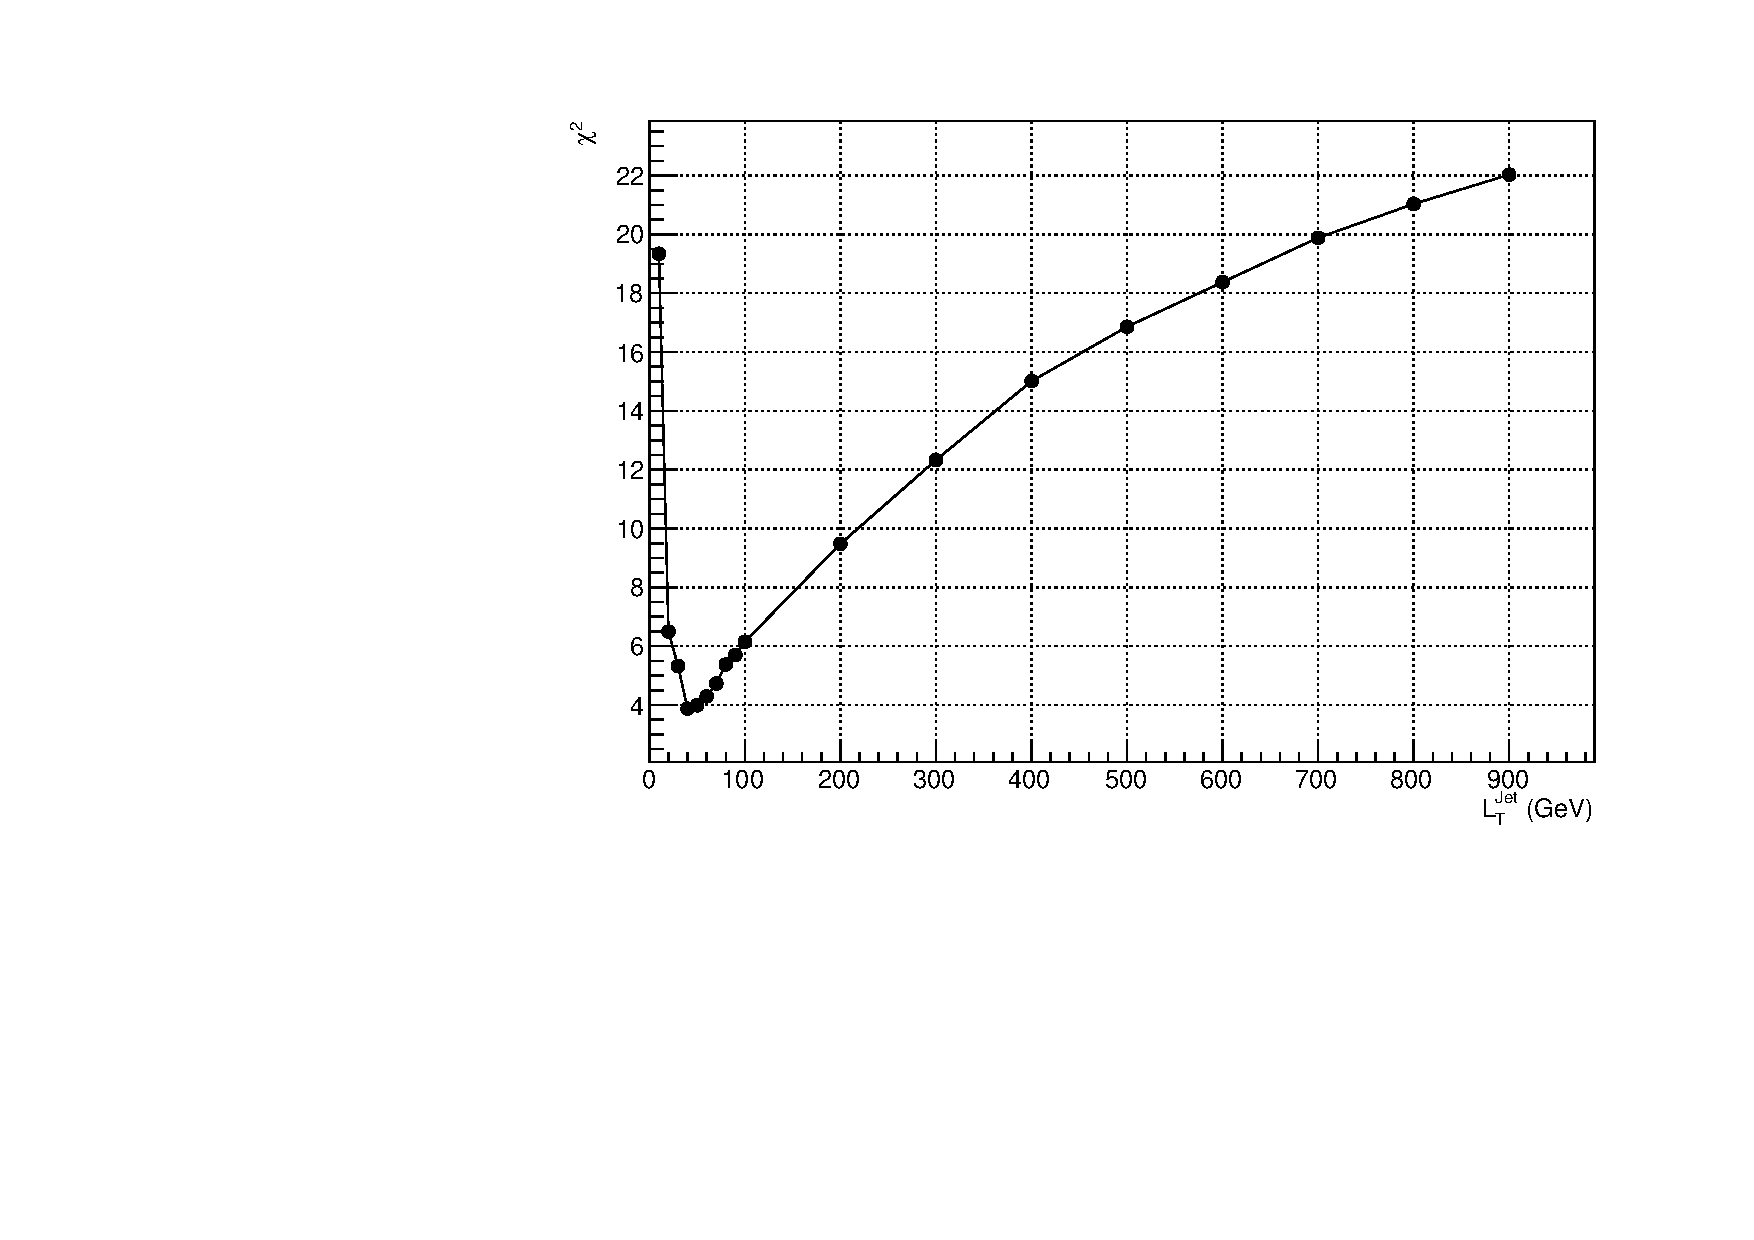
\includegraphics[width=0.5\textwidth]{4_Analisys/pics/8TeV/ProfileNeighbors/MM/h2taucuts/LT_chi2.pdf}
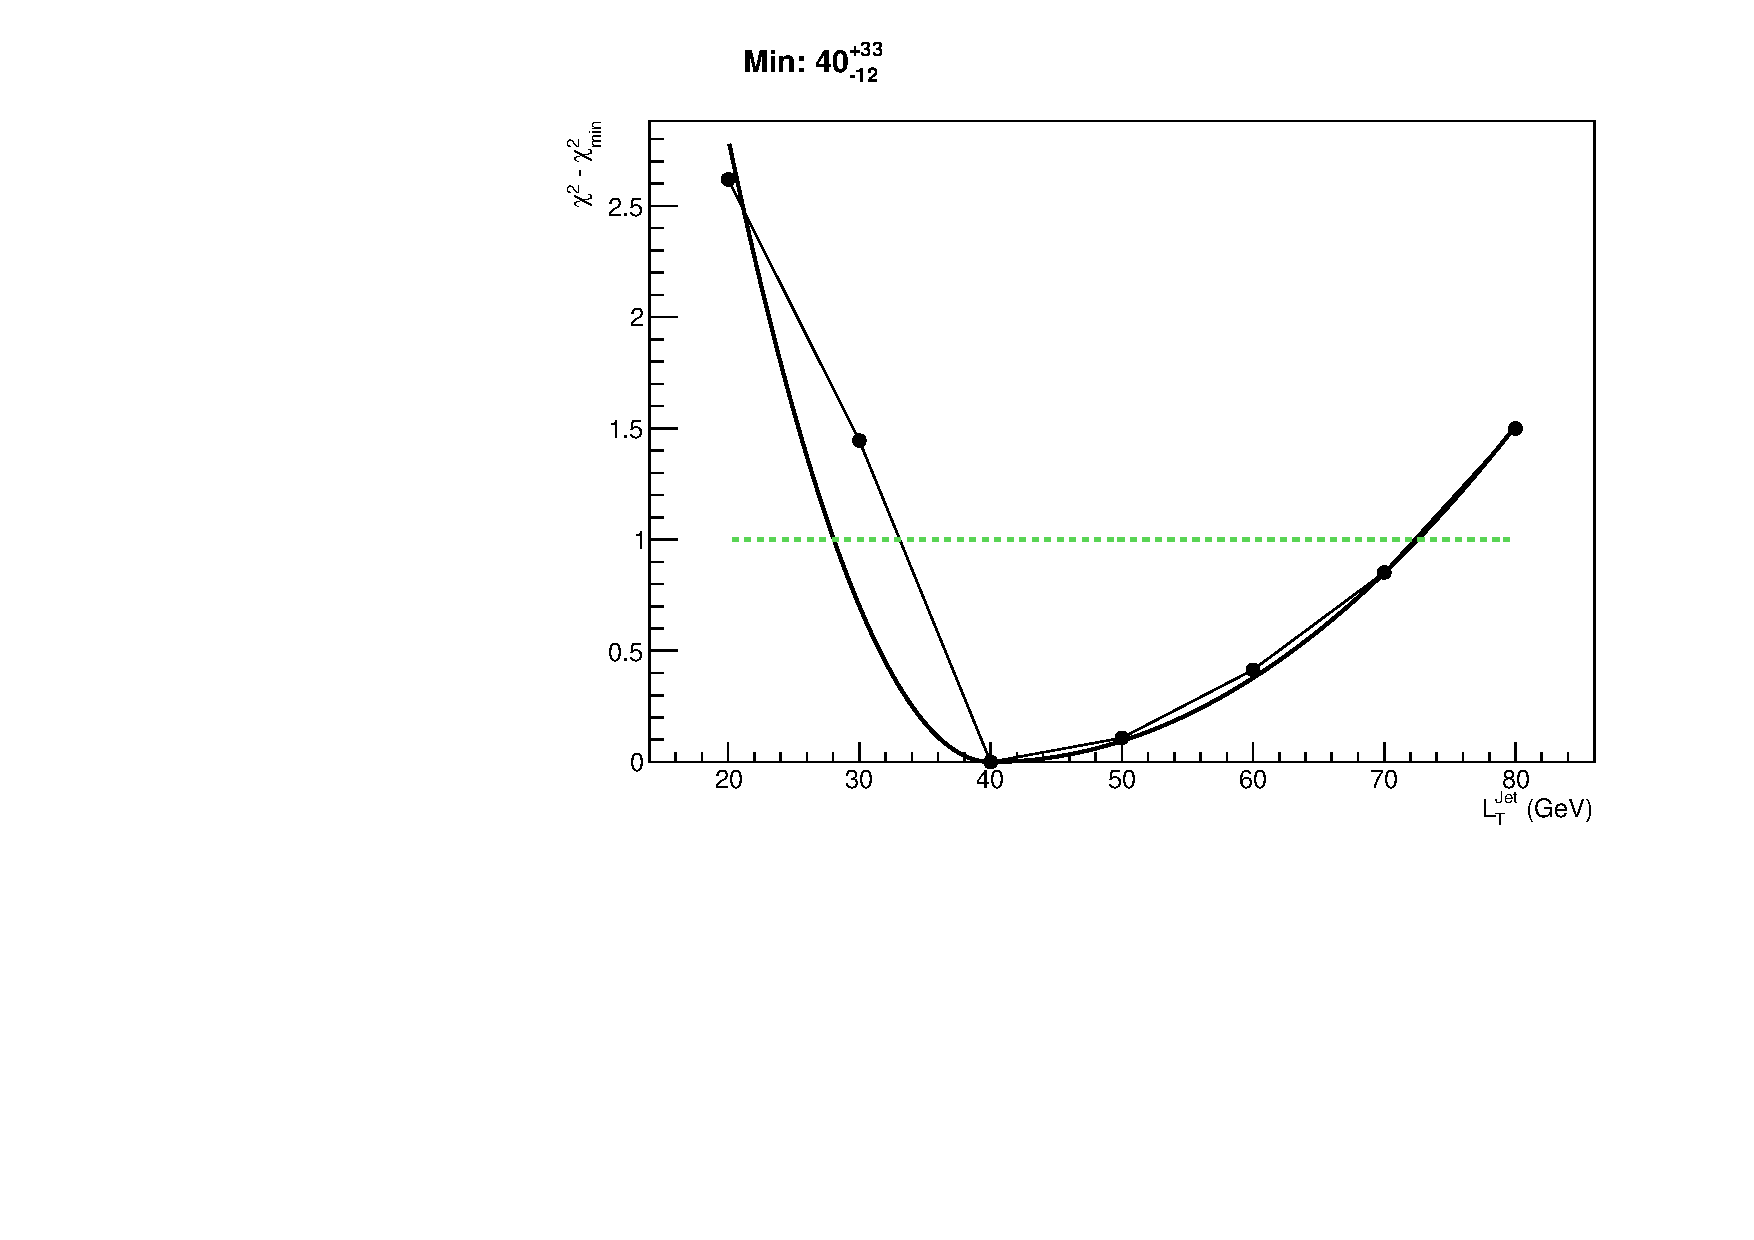
\includegraphics[width=0.5\textwidth]{4_Analisys/pics/8TeV/ProfileNeighbors/MM/h2taucuts_LT.pdf} \\
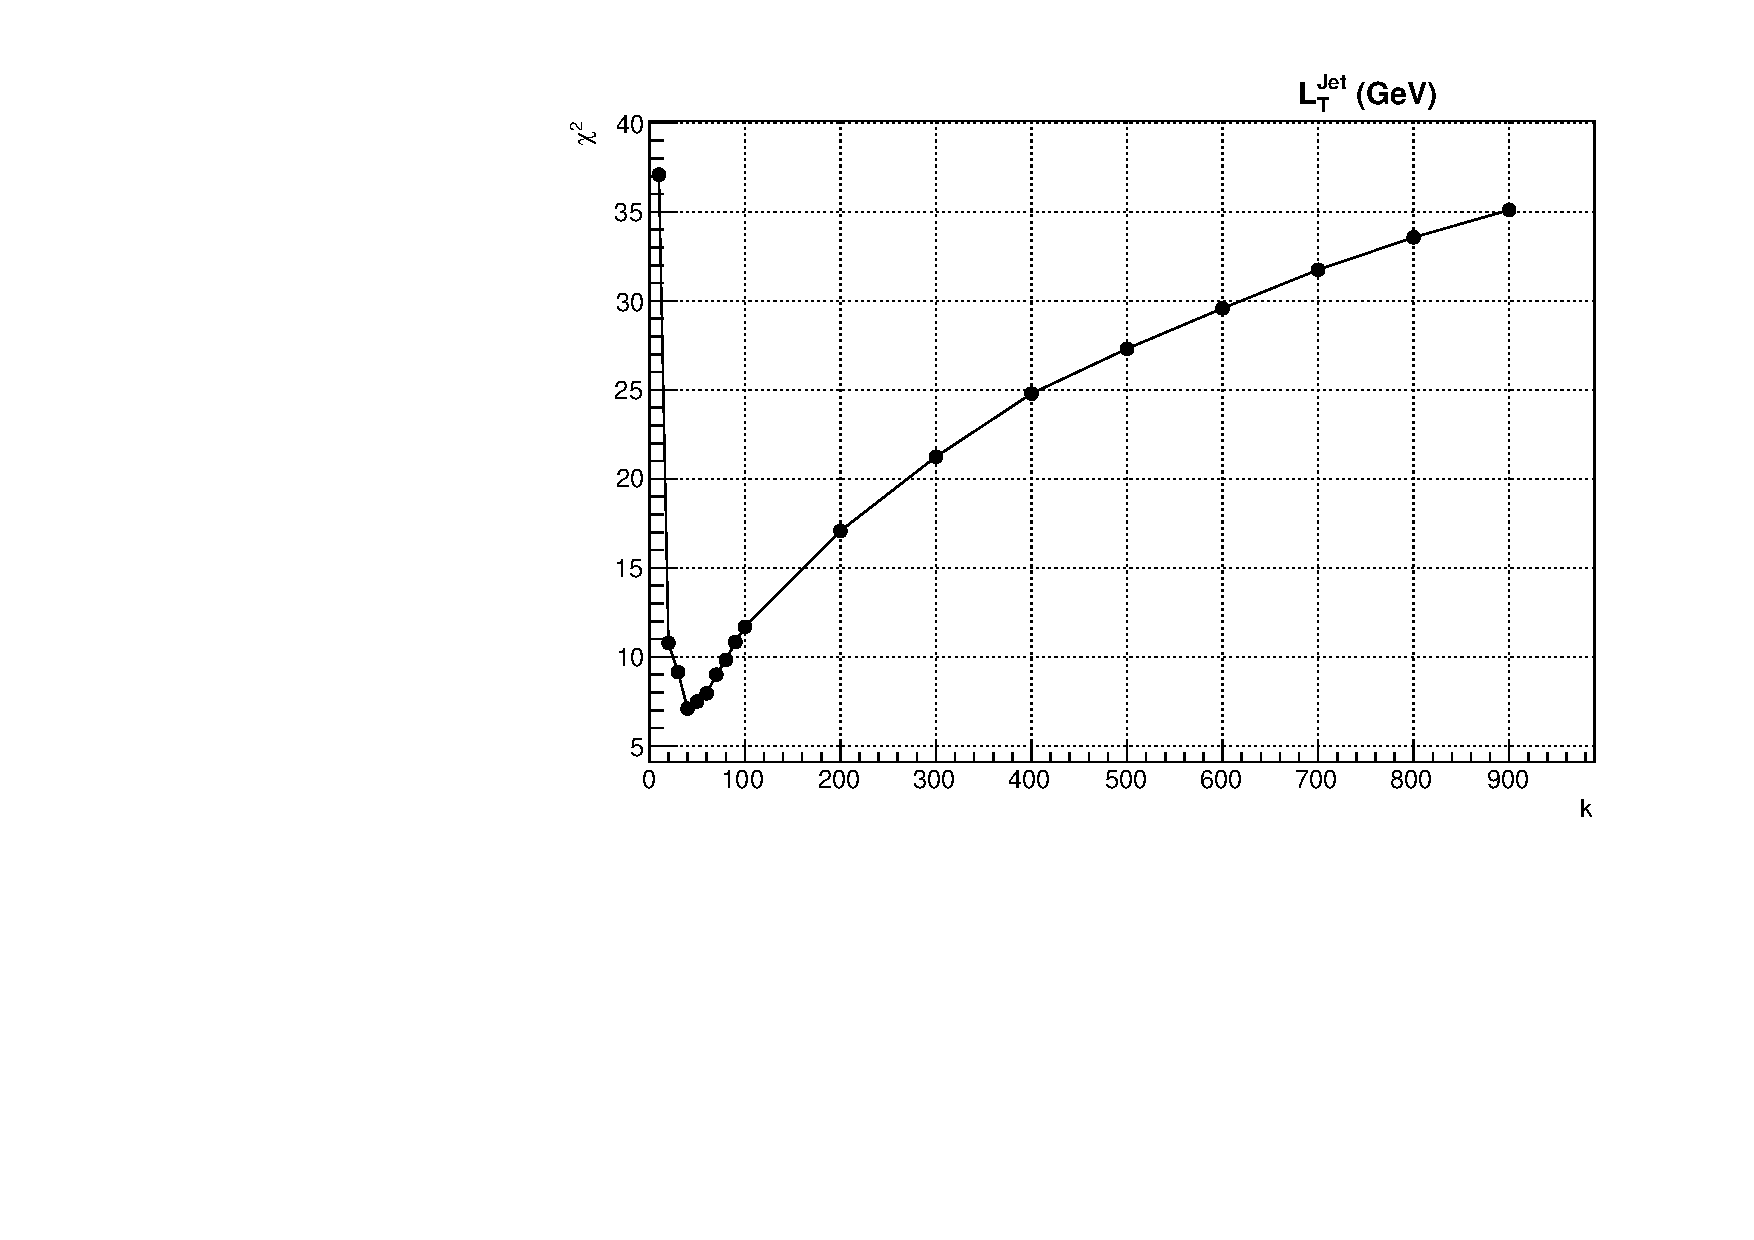
\includegraphics[width=0.5\textwidth]{4_Analisys/pics/8TeV/ProfileNeighbors/MM/h2taucuts020/LT_chi2.pdf}
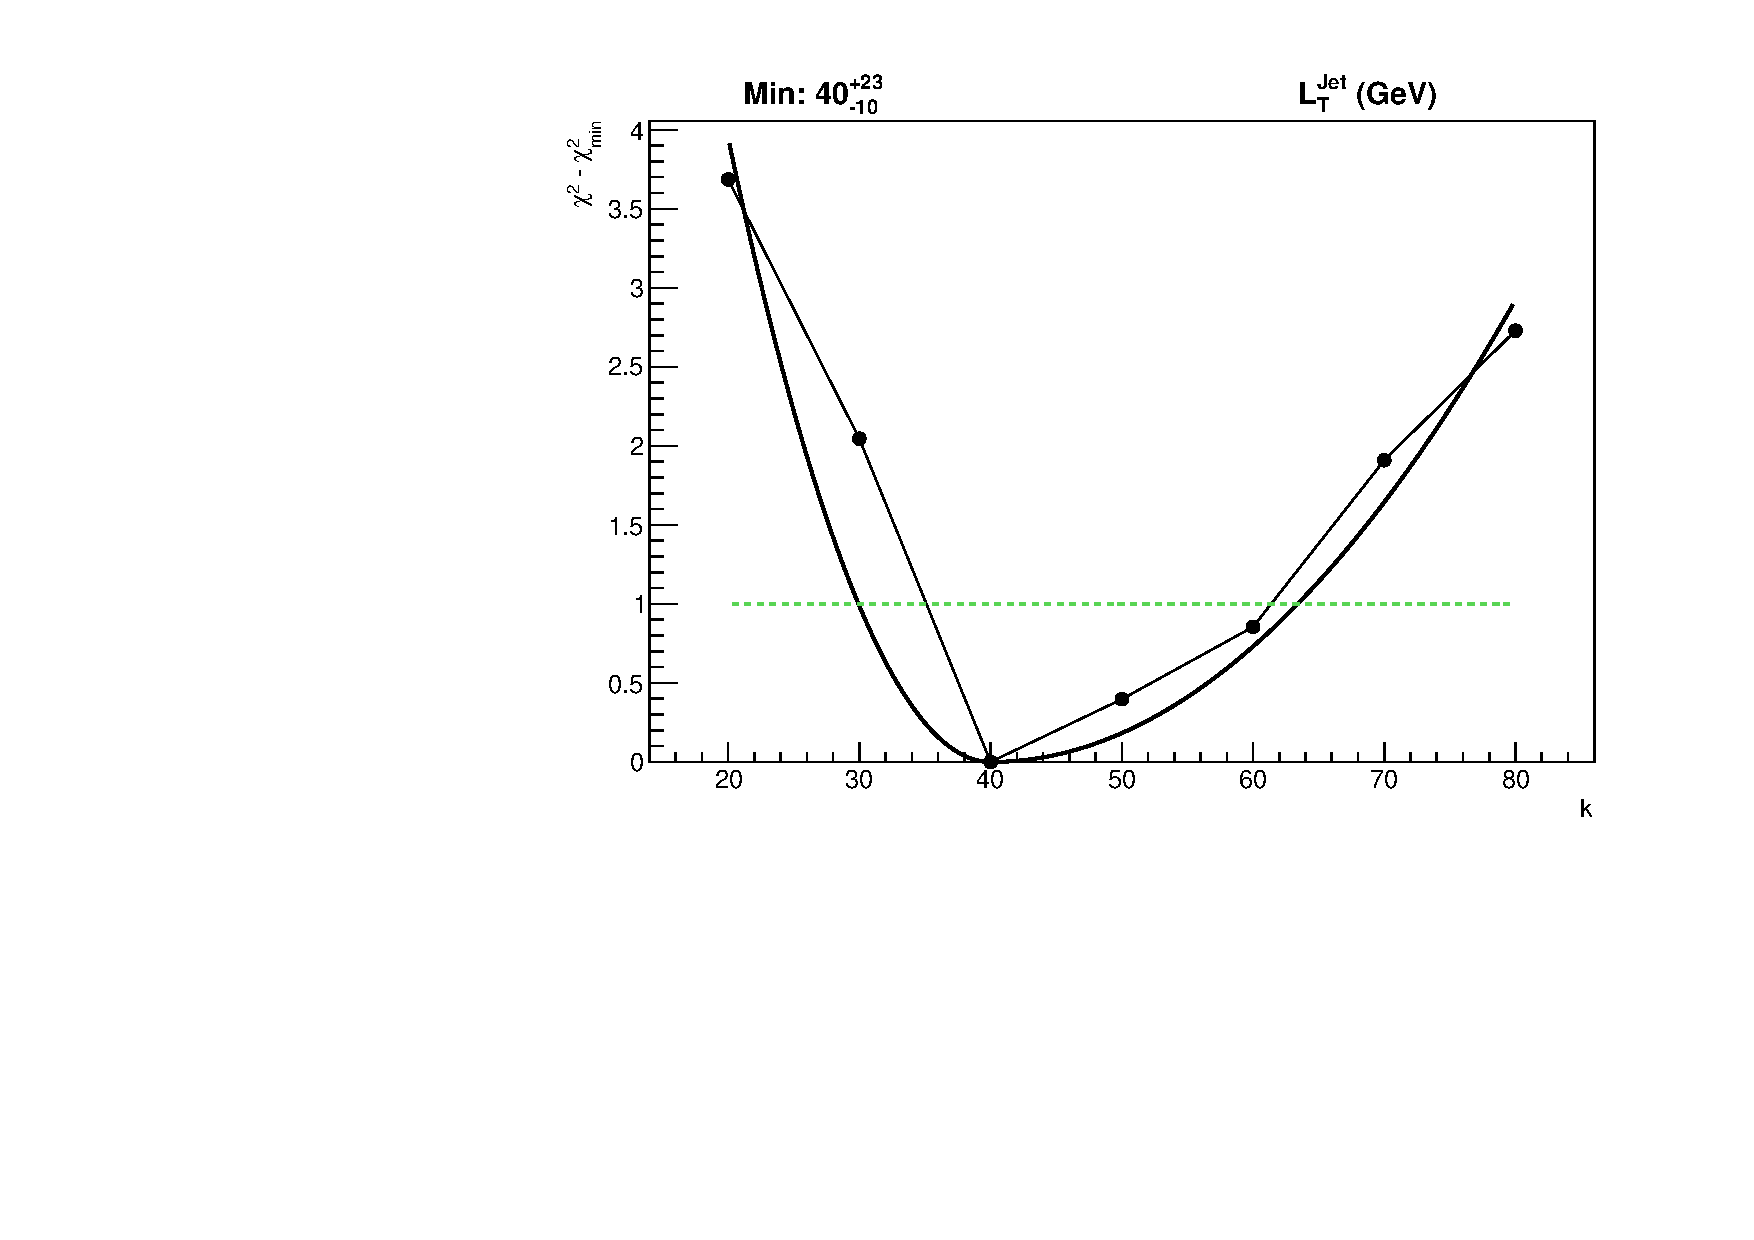
\includegraphics[width=0.5\textwidth]{4_Analisys/pics/8TeV/ProfileNeighbors/MM/h2taucuts020_LT.pdf} \\
\caption{\chisq scan of different neighbors value (left) and corresponding minima fit (right) for leading (top) and sub-leading (bottom) muons in $\mu\mu\tau_h$ channel. The variable used for the scan is the scalar sum of the \pT of the two leptons and the jet}
\label{fig:kNN_minima_MMT}
\end{figure}

\begin{figure}
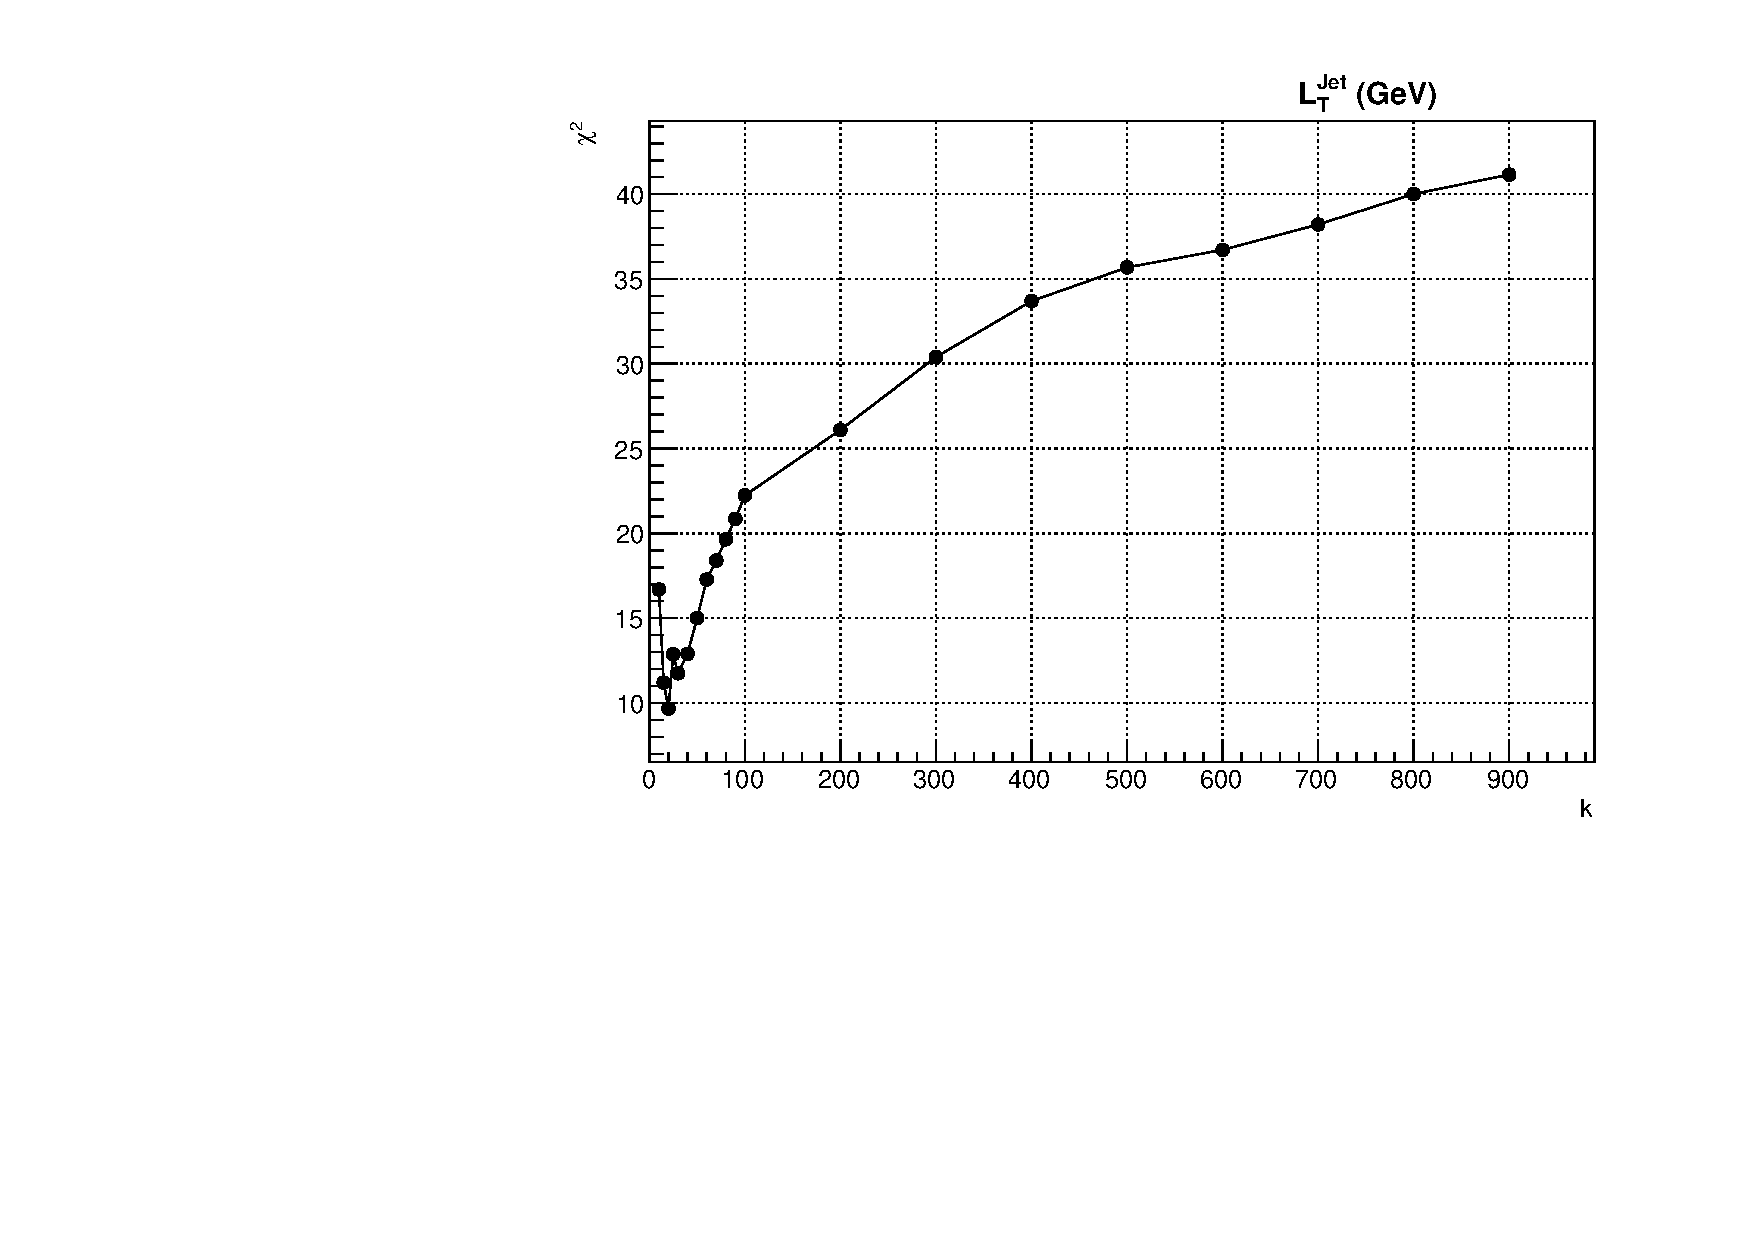
\includegraphics[width=0.5\textwidth]{4_Analisys/pics/8TeV/ProfileNeighbors/EM_Muon/h2taucuts/LT_chi2.pdf}
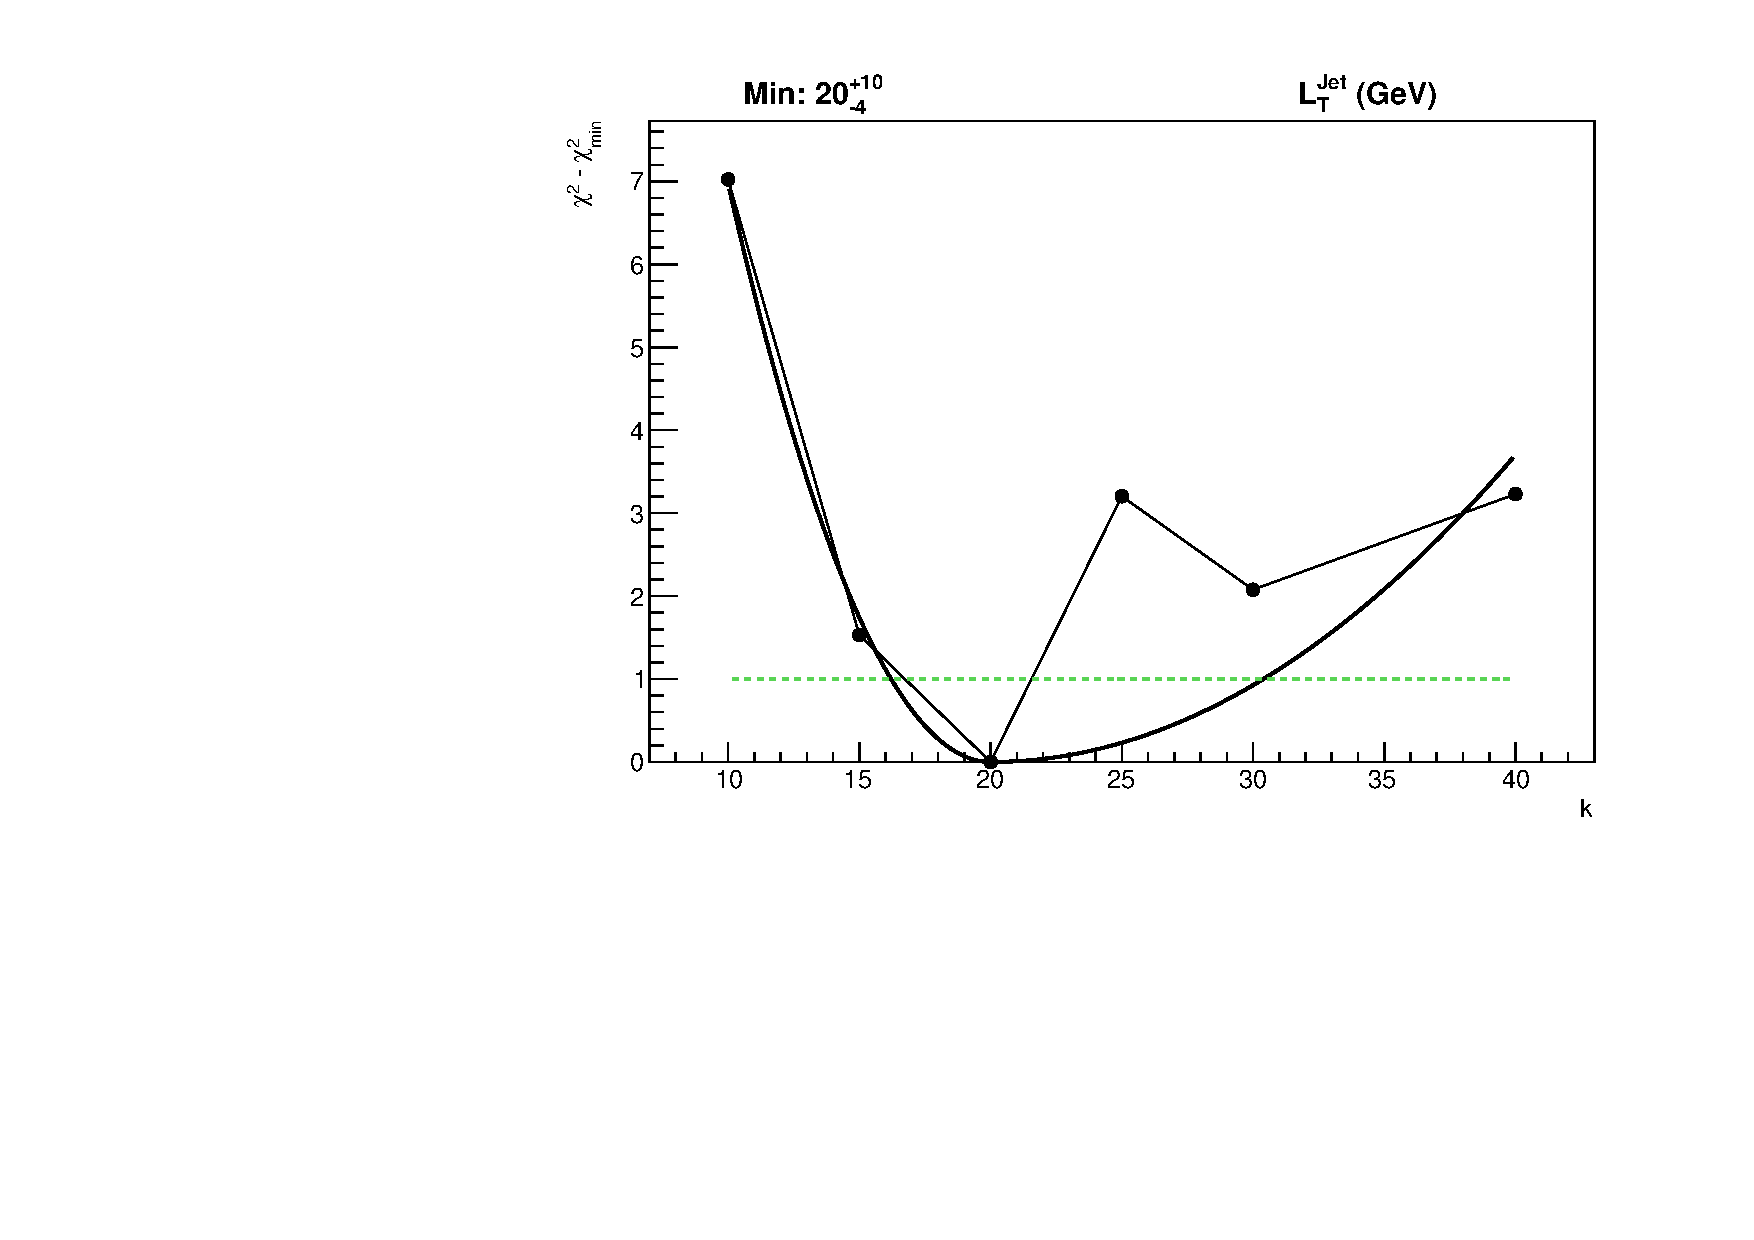
\includegraphics[width=0.5\textwidth]{4_Analisys/pics/8TeV/ProfileNeighbors/EM_Muon/h2taucuts_LT.pdf} \\
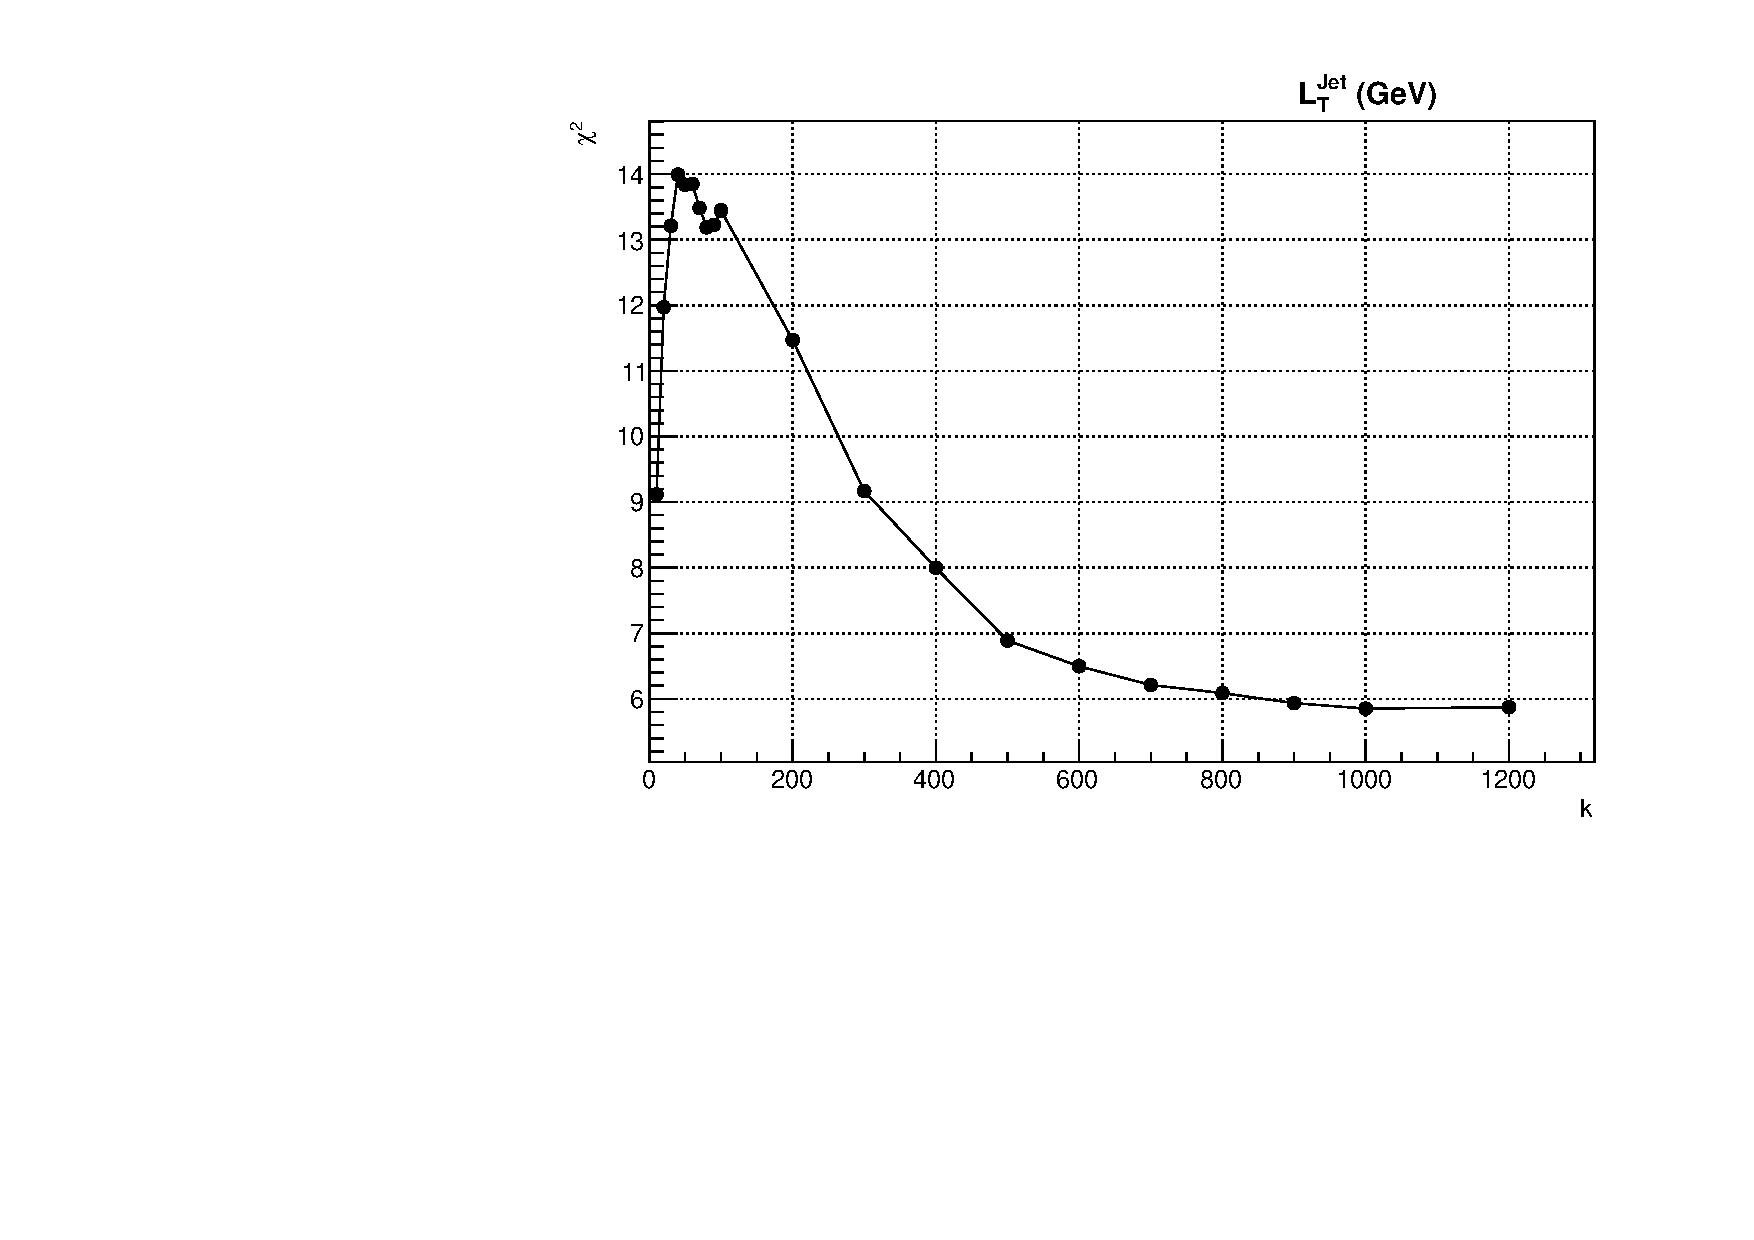
\includegraphics[width=0.5\textwidth]{4_Analisys/pics/8TeV/ProfileNeighbors/EM_Electron/eid12Medium_h2taucuts/LT_chi2.pdf}
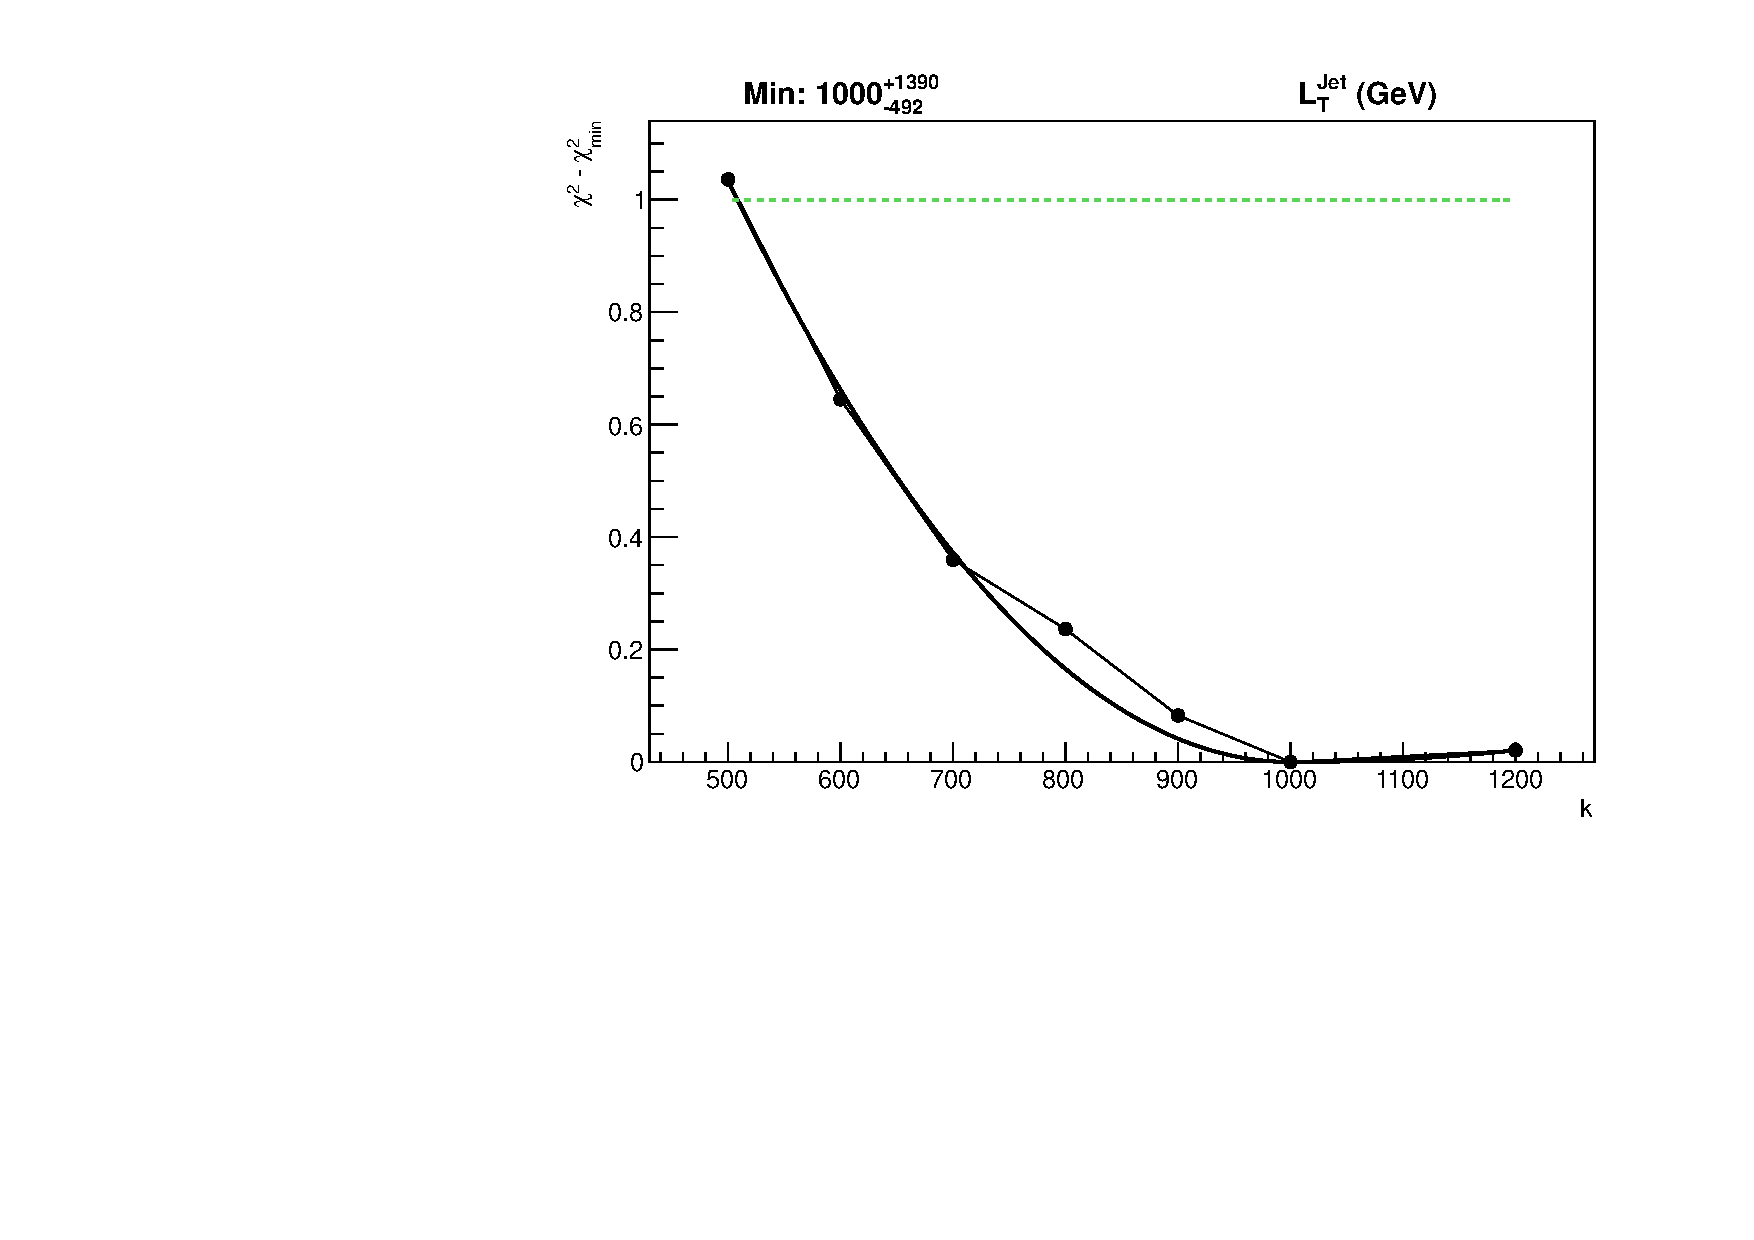
\includegraphics[width=0.5\textwidth]{4_Analisys/pics/8TeV/ProfileNeighbors/EM_Electron/eid12Medium_h2taucuts_LT.pdf} \\
\caption{\chisq scan of different neighbors value (left) and corresponding minima fit (right) for muon (top) and electron (bottom) in $e\mu\tau_h$ channel. The variable used for the scan is the scalar sum of the \pT of the two leptons and the jet}
\label{fig:kNN_minima_EMT}
\end{figure}

\begin{figure}
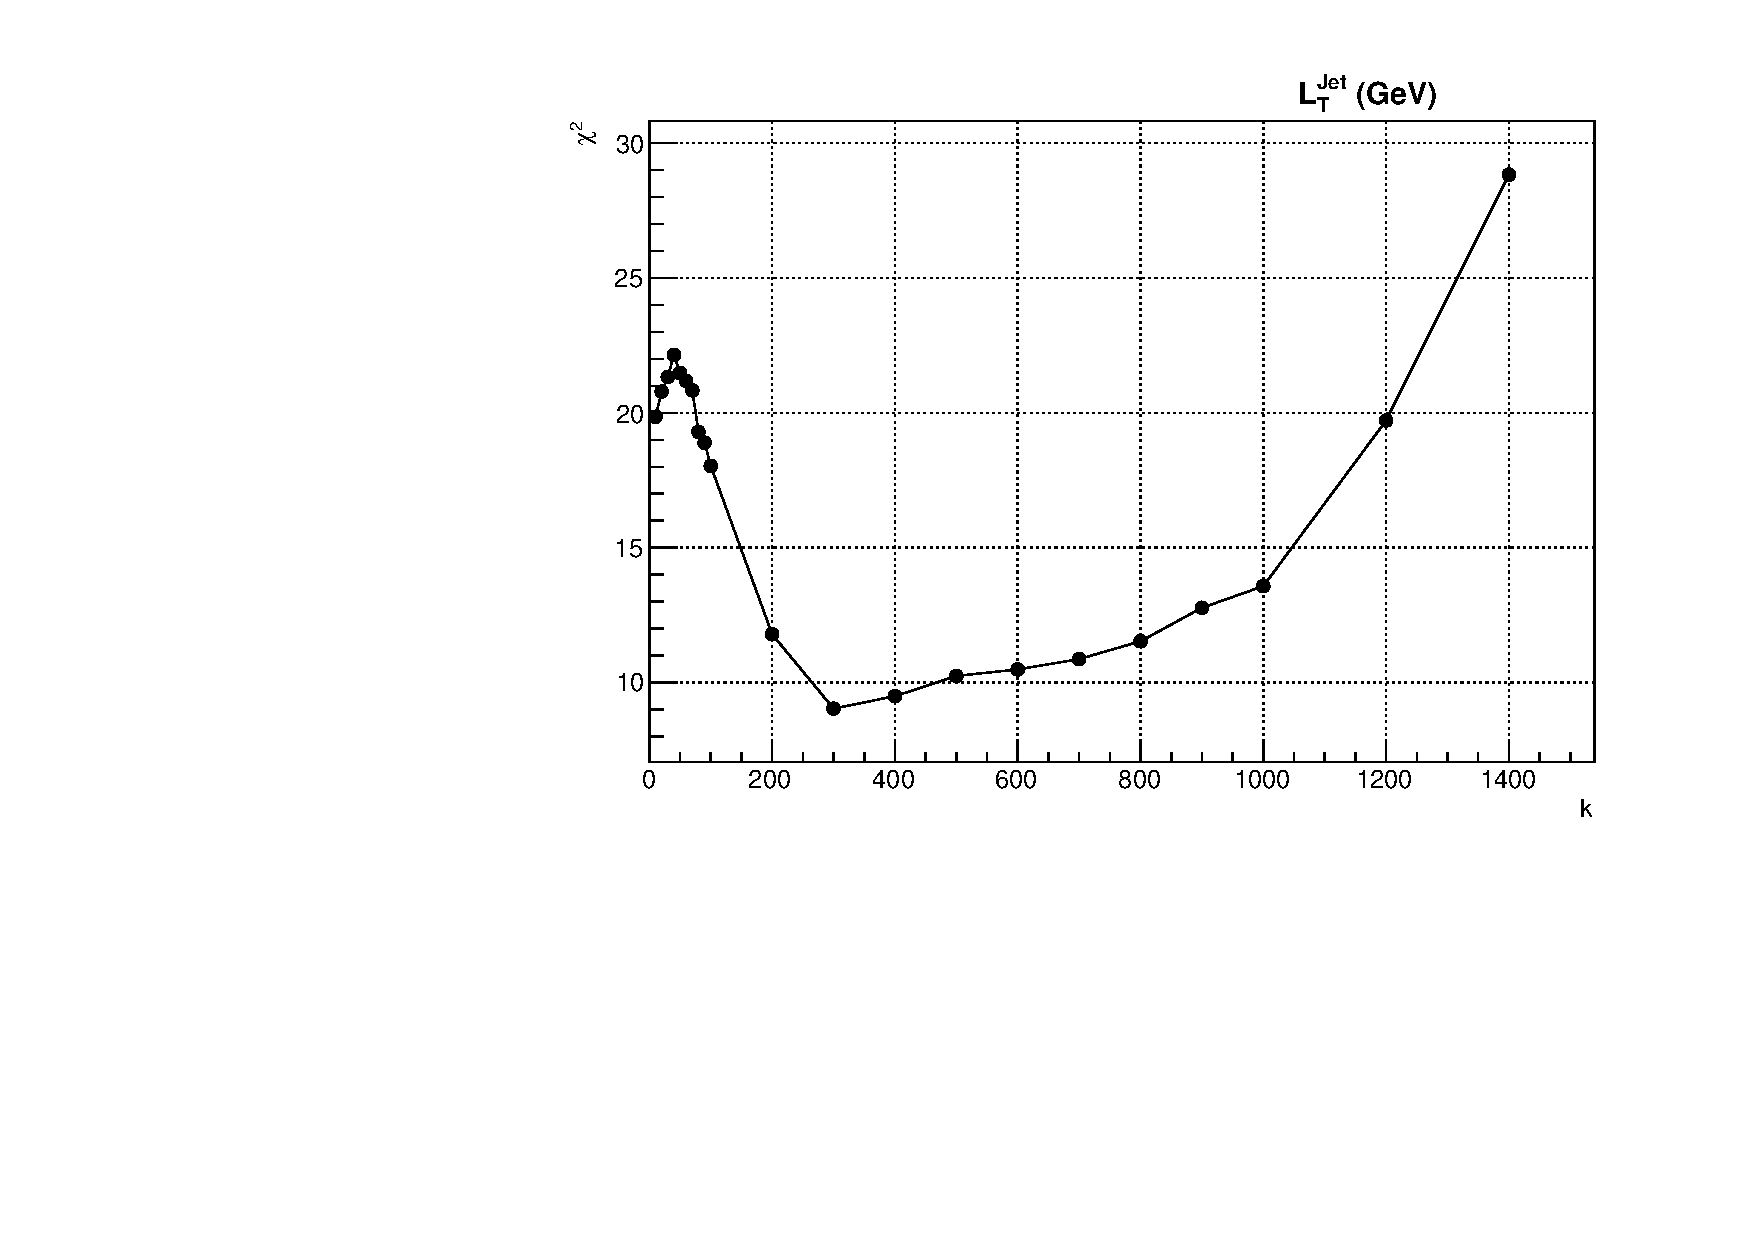
\includegraphics[width=0.5\textwidth]{4_Analisys/pics/8TeV/ProfileNeighbors/EE/eid12Tight_h2taucuts/LT_chi2.pdf}
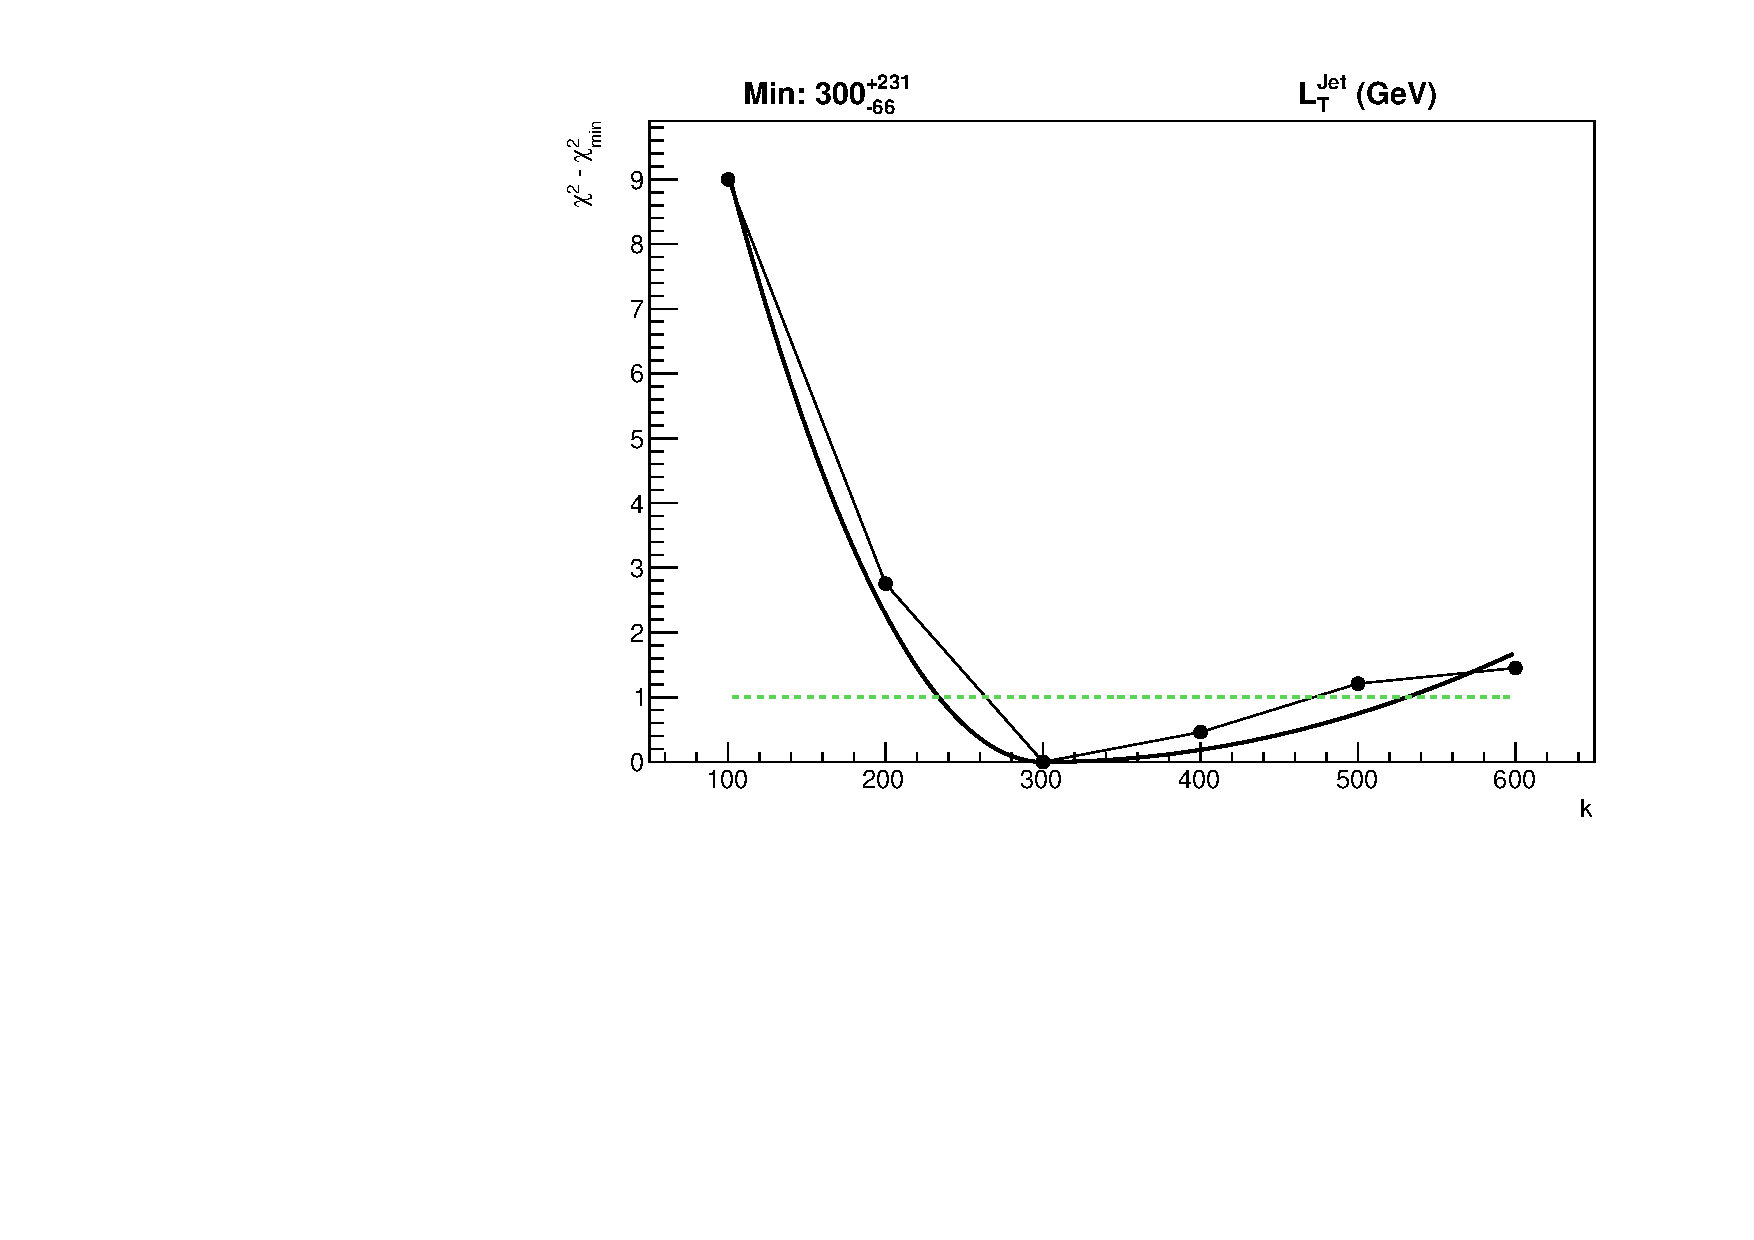
\includegraphics[width=0.5\textwidth]{4_Analisys/pics/8TeV/ProfileNeighbors/EE/eid12Tight_h2taucuts_LT.pdf} \\
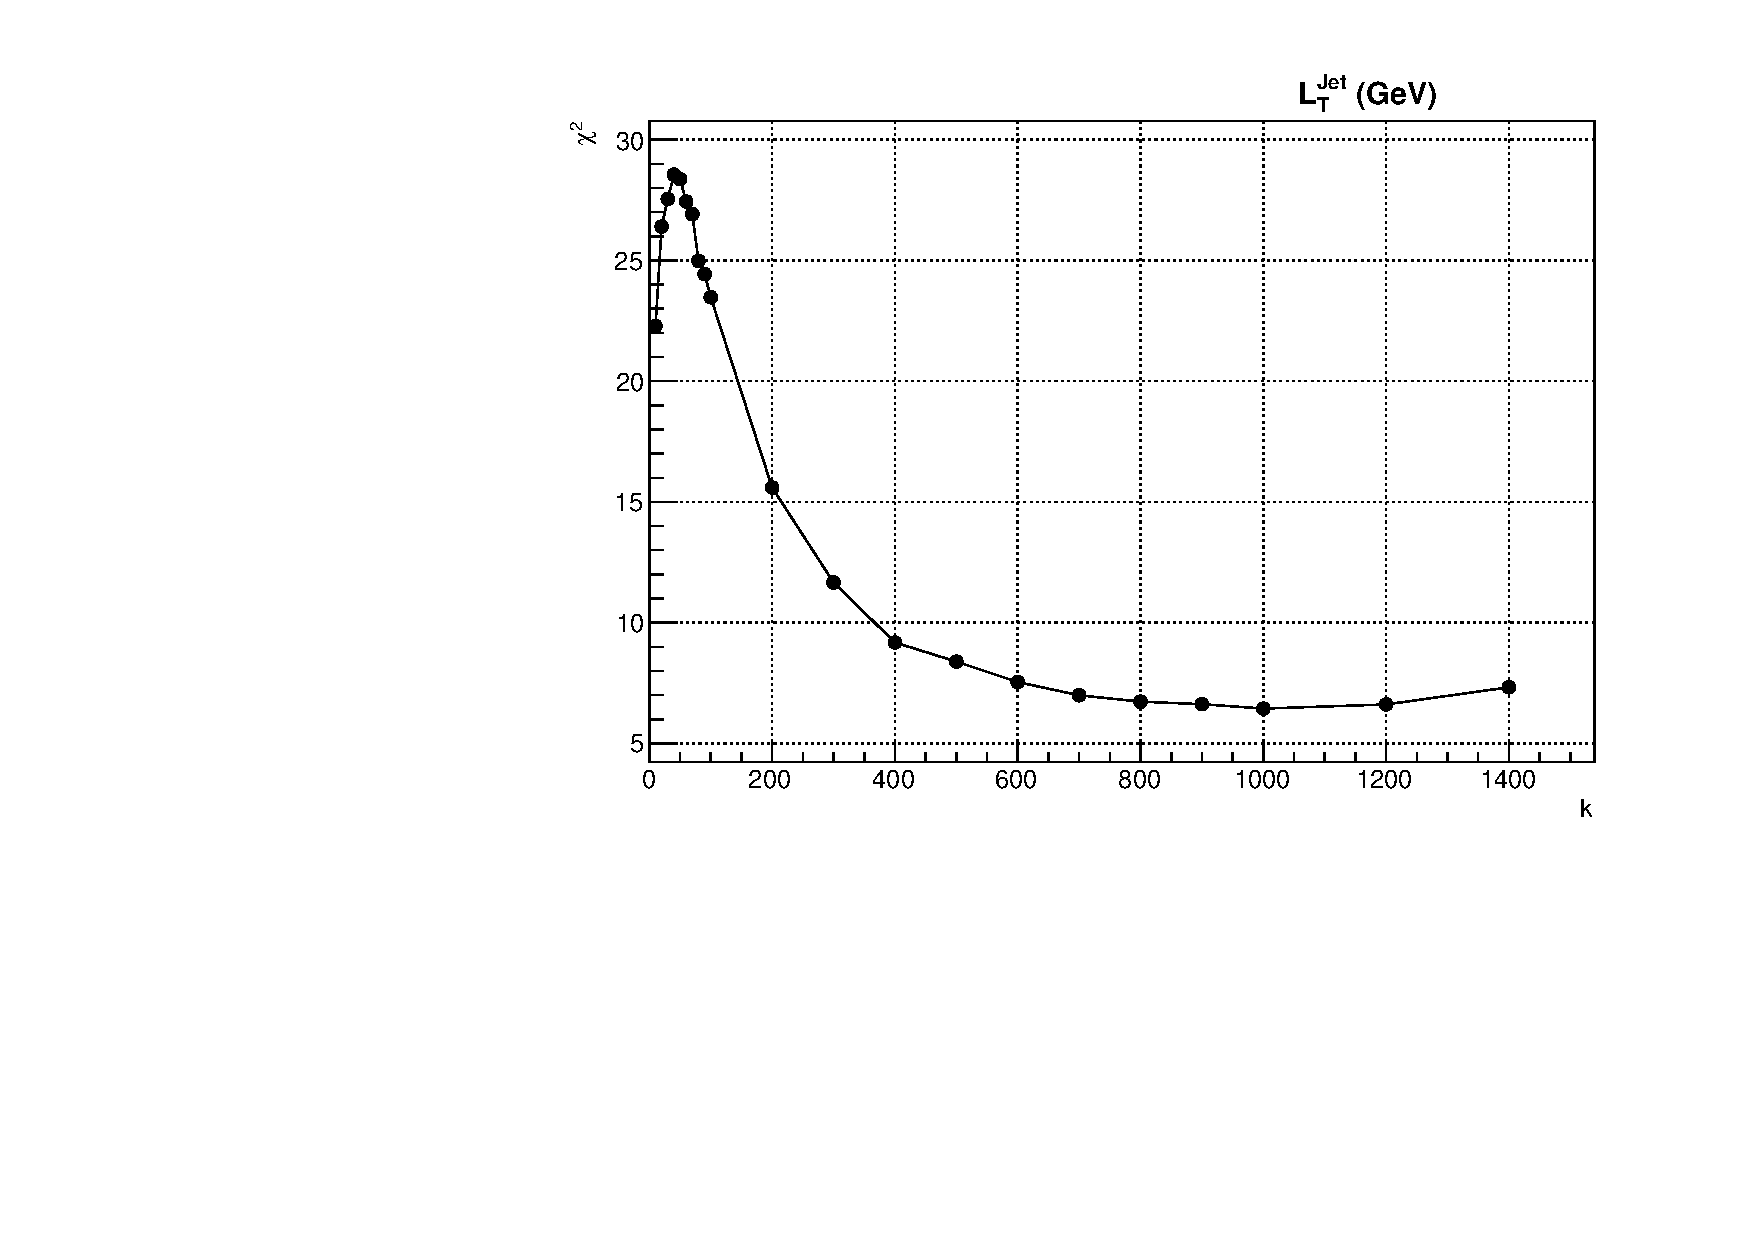
\includegraphics[width=0.5\textwidth]{4_Analisys/pics/8TeV/ProfileNeighbors/EE/eid12Medium_h2taucuts020/LT_chi2.pdf}
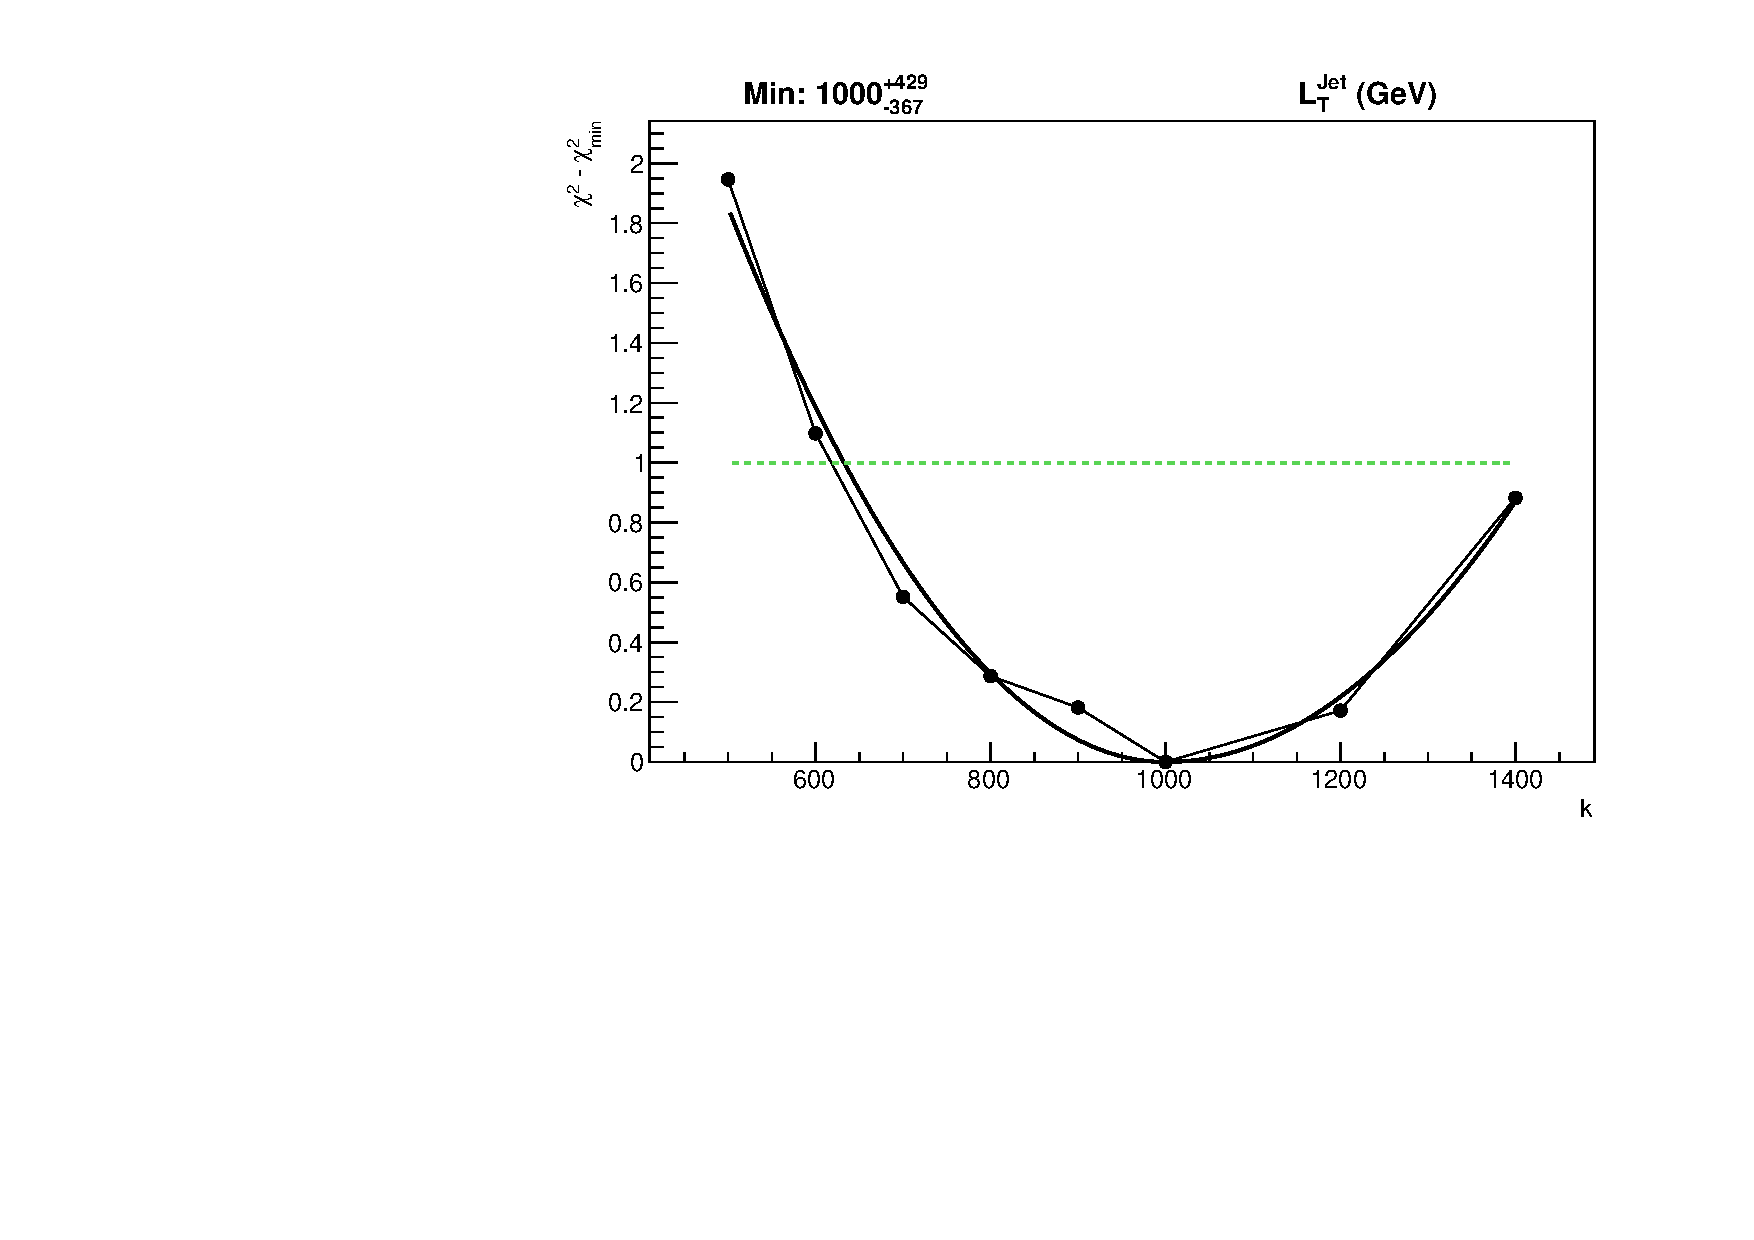
\includegraphics[width=0.5\textwidth]{4_Analisys/pics/8TeV/ProfileNeighbors/EE/eid12Medium_h2taucuts020_LT.pdf} \\
\caption{\chisq scan of different neighbors value (left) and corresponding minima fit (right) for leading (top) and sub-leading (bottom) electrons in $ee\tau_h$ channel. The variable used for the scan is the scalar sum of the \pT of the two leptons and the jet}
\label{fig:kNN_minima_EET}
\end{figure}

